% !TEX TS-program = LuaLaTeX
\documentclass[11pt,compress,xcolor=x11names,UTF8]{beamer}
\usetheme{Boadilla}
\usecolortheme{seahorse}
\useinnertheme[shadow]{rounded}
\useoutertheme[subsection=false]{smoothbars}
\usecolortheme{spruce}
\usecolortheme[named=SpringGreen4]{structure}
\usefonttheme{structurebold}
\useinnertheme{circles}
\usecolortheme{rose}
\usepackage{pifont}
\usepackage{academicons}
\usepackage{fontawesome}
\usepackage{iitem}
\usepackage{graphicx}
\usepackage{tabularx}
\usepackage{ gensymb }
\setbeamertemplate{itemize item}{\ding{108}}
\setbeamertemplate{itemize subitem}{\ding{109}}
\setbeamertemplate{navigation symbols}{}
\setbeamercovered{transparent}
\renewcommand\appendixname{附录}
\renewcommand\abstractname{摘要}
\graphicspath{{figure/}} % 图片路径
\usepackage{calligra} % Thank you
\usepackage{ctex} % 加入中文
%\setCJKsansfont{Noto Sans CJK SC}
\setsansfont{Lato} % Lato Roboto Fira Sans
\usepackage{makecell}
\newcommand{\tabincell}[2]{\begin{tabular}{@{}#1@{}}#2\end{tabular}}
\usepackage{url}
\usepackage{natbib} % 参考文献
%\title[Spatial Generalized Linear Mixed Models]{Spatial Generalized Linear Mixed Models with Application to Prevalence Mapping}
\title{Detector Simulation Using GEANT4}
%\subtitle{奖助金申请答辩}
\author[Rong Zhao]{Email:zhaor25@mail2.sysu.edu.cn \and  } % \\ 专业:统计学 \\ 方向:数据分析与统计计算
\institute[SYSU]{School of Physics\and } % 理学院\\
\date[\today]{
\includegraphics[width=.5\textwidth]{logo}}

\begin{document}

\maketitle

\begin{frame}{Outline}
\tableofcontents
\end{frame}

\section{Brief Introduction}

%\subsection{研究意义}

\begin{frame}{Priliminary Geometry Design}
\begin{enumerate}
\item scintillator cubes $10\times 10 \times 10$
\item flat film as neutron detector: 4layers
\item six light guide arrays
\item six PMT [SiPM] arrays
\end{enumerate}
\vspace{-1cm}
\begin{columns}
\begin{column}{.33\textwidth}
\begin{figure}
\centering
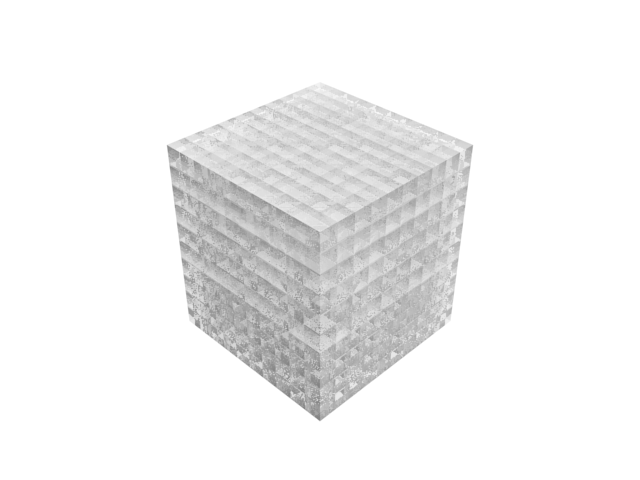
\includegraphics[width=1.3\textwidth]{currentfig/geo1.png} % 单图
%\label{fig:wave2d}
\caption{scintillator \qquad \qquad \qquad cube}
\end{figure}
\end{column}
\begin{column}{.33\textwidth}
\begin{figure}
\centering
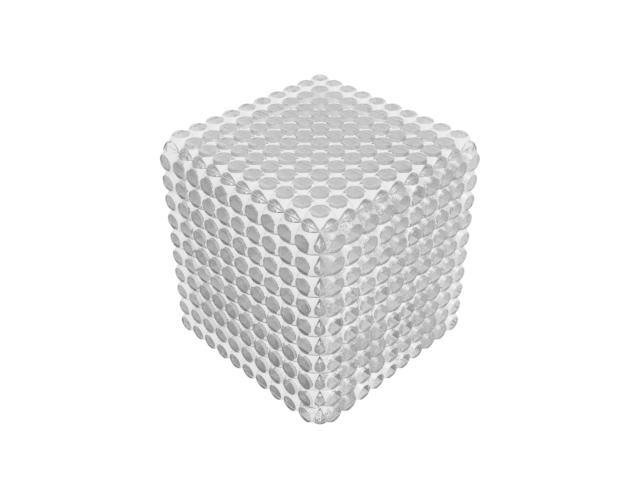
\includegraphics[width=1.25\textwidth]{currentfig/geo2.png} % 单图
\caption{scintillator cube+light guide}
\end{figure}
\end{column}
\begin{column}{.33\textwidth}
\begin{figure}
\centering
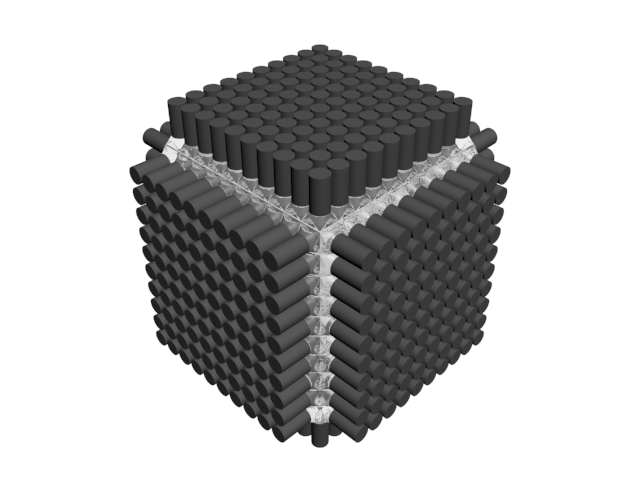
\includegraphics[width=1.2\textwidth]{currentfig/geo3.png} % 单图
%\label{fig:wave2d}
\caption{scintillator cube+light guide+PMT}
\end{figure}
\end{column}
\end{columns}
\end{frame}

\begin{frame}{Details about the Geometry Set-up}
%\textsf{例} \textbf{例}  \textit{例}
% \texttt{例}  % 调出仿宋字体了
%The cubic detector contains 10$\times$10$\times$10 small scintillators with size 6cm$\times$6cm$\times$6cm; two arrays of SiPMs is 1mm away from the scintillator surface.
The structure of one dimention detector:
\begin{columns}
\begin{column}{1.05\textwidth}
\begin{figure}
\centering
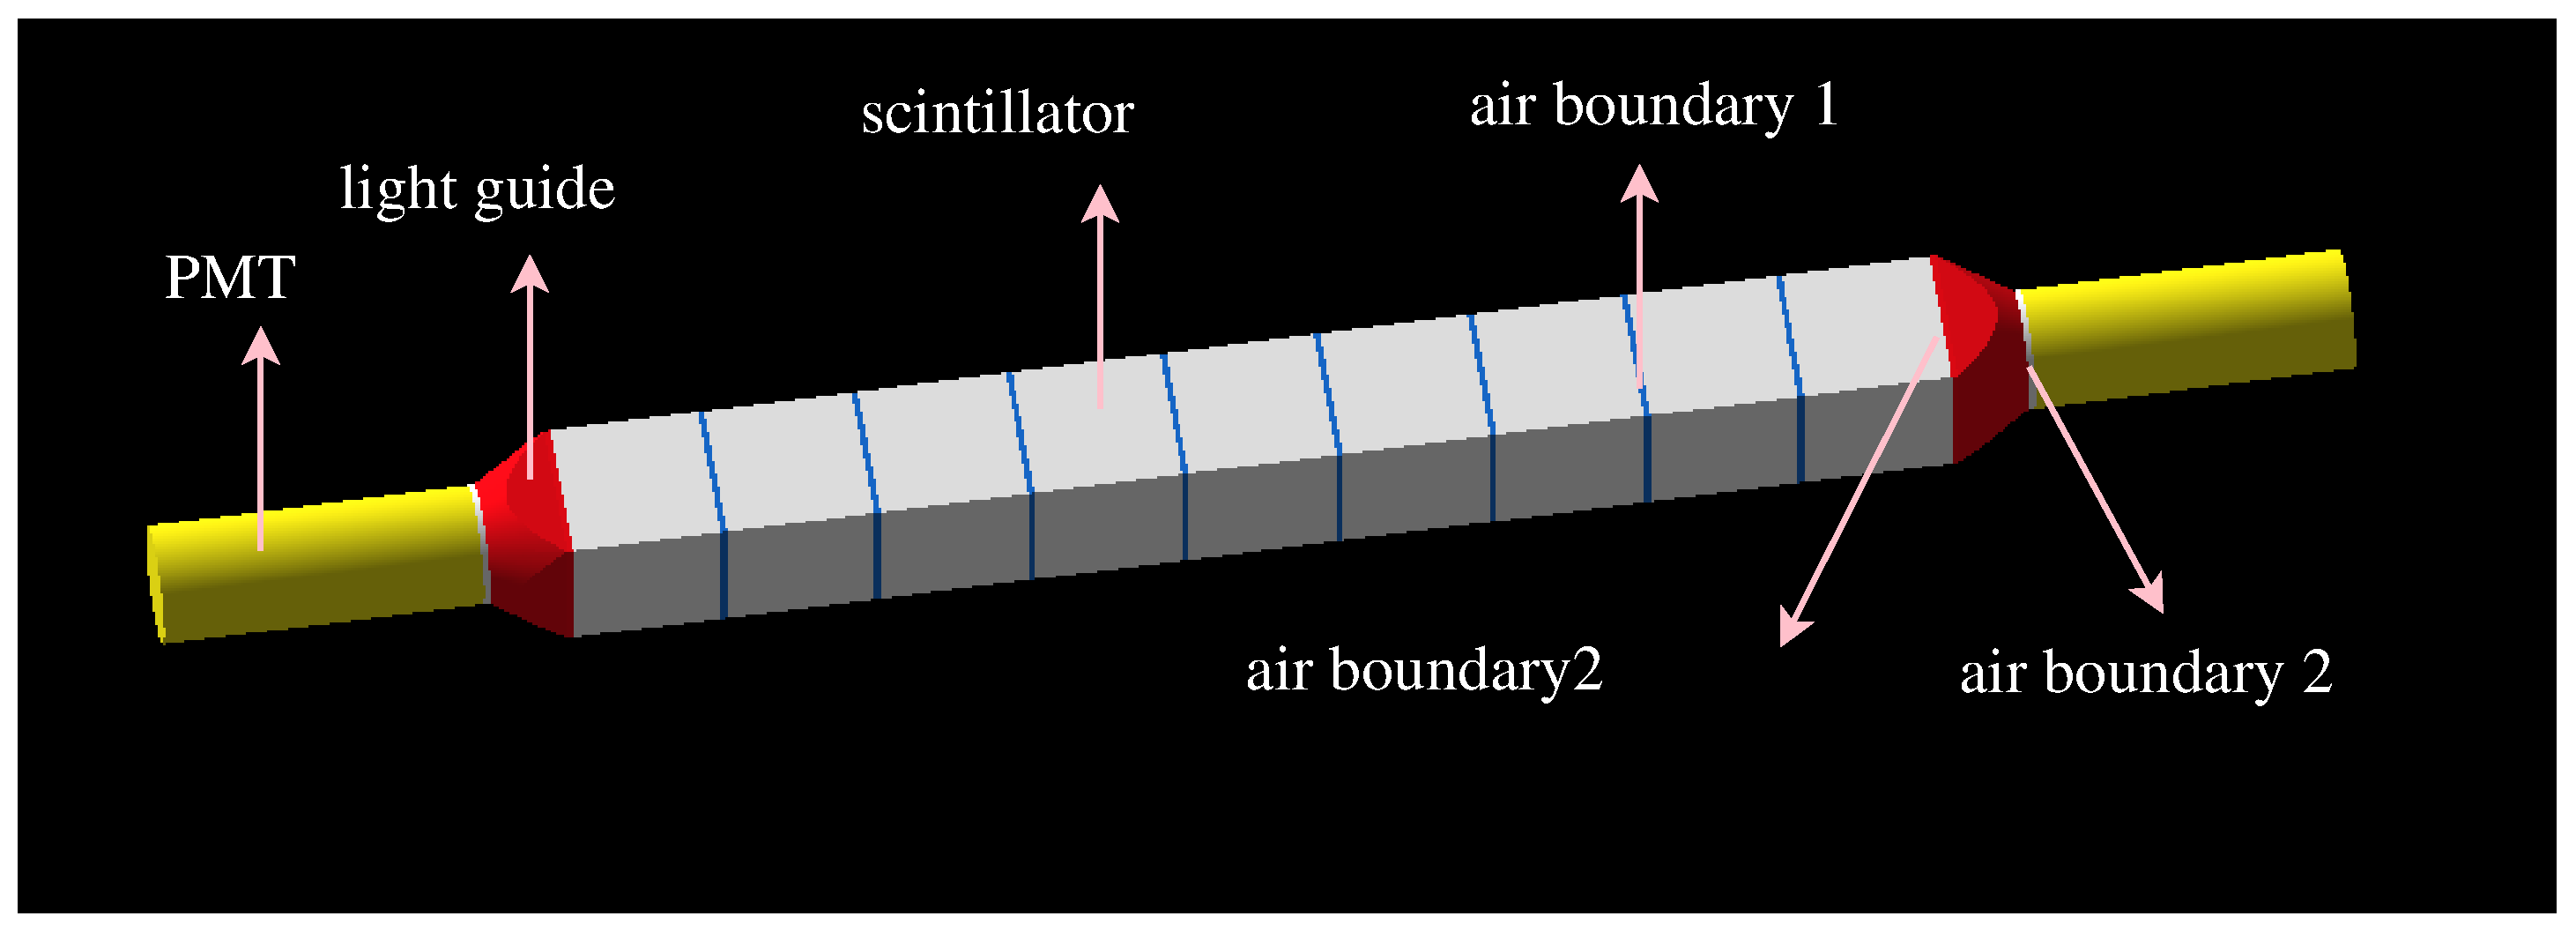
\includegraphics[width=\textwidth]{currentfig/onedim.eps} % 单图
%\label{fig:wave2d}
\caption{Geometry structure:PMT-lightguide-scintillator-air boundary between [scintillators;scintillator and lightguide;lightguide and PMT cathode] }
\end{figure}
\end{column}
%\begin{column}{.5\textwidth}
%\begin{figure}
%\centering
%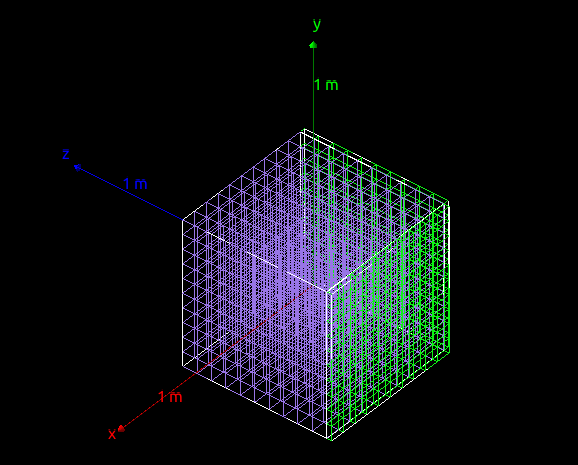
\includegraphics[width=.99\textwidth]{currentfig/geom2.png} % 单图
%%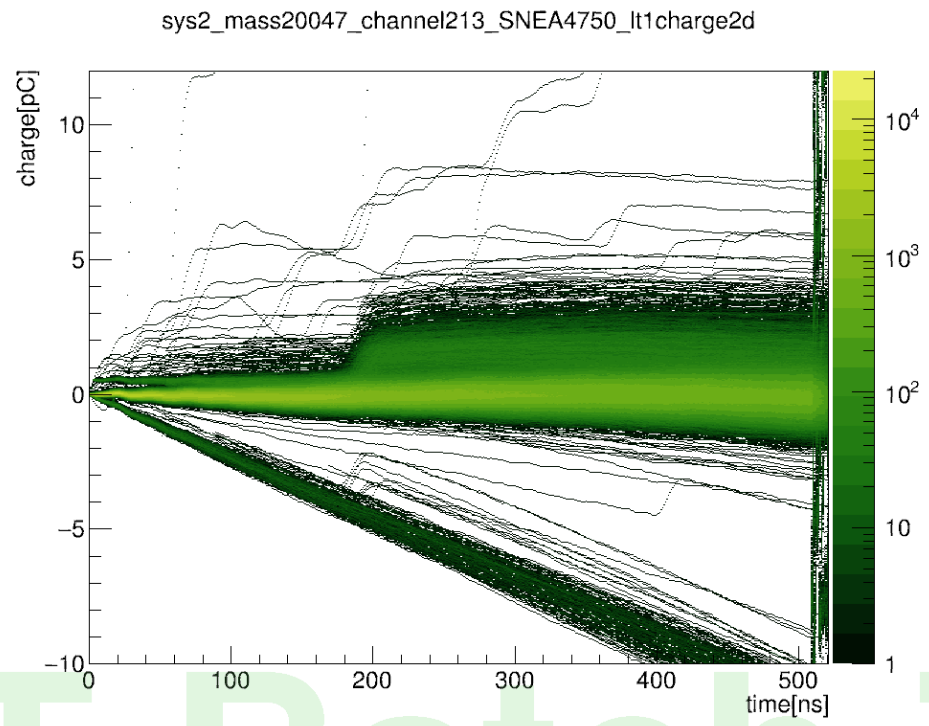
\includegraphics[width=\textwidth]{figures/baseline2d.png} % 单图
%\caption{geometry of detector}
%\end{figure}
%\end{column}
\end{columns}
\end{frame}
%%%%%%%%%%%%%%%%%%%%%%%%%%%%%%%%%%%%%%%%%%%%%%%%%%%%%%%%%%%%
\begin{frame}{Details about the Geometry Set-up}
%\begin{frame}{detailed geometry options}
\begin{figure}
\centering
\includegraphics[width=.75\textwidth]{currentfig/twodim.eps} % 单图
%\label{fig:wave2d}
\caption{two dimention detector layout}
\end{figure}

\end{frame}
%%%%%%%%%%%%%%%%%%%%%%%%%%%%%%%%%%%%%%%%%%%%%%%%%%%%%%%%%%%%
\begin{frame}{Details about the Geometry Set-up}
Not finished yet.
%\begin{frame}{detailed geometry options}
\begin{figure}
\centering
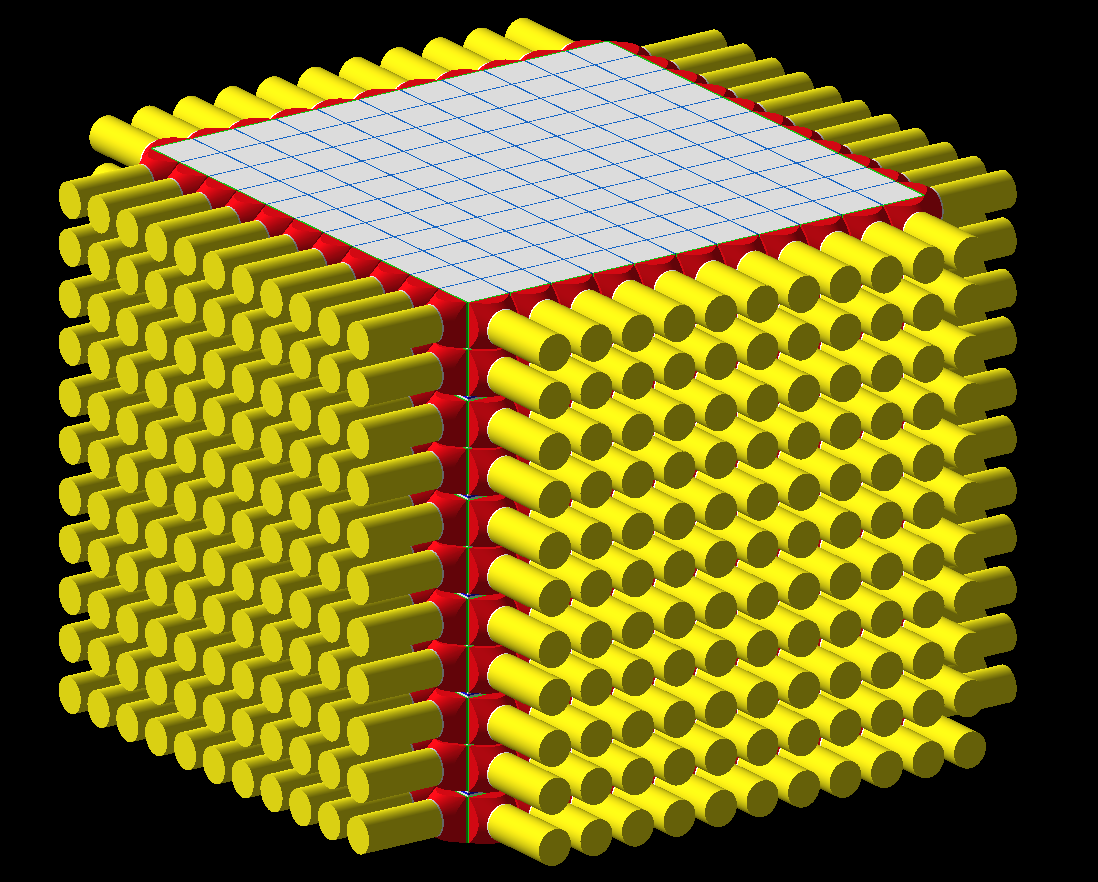
\includegraphics[width=.55\textwidth]{currentfig/3dg.eps} % 单图
%\label{fig:wave2d}
\caption{3 dimention detector layout}
\end{figure}
\end{frame}
%%%%%%%%%%%%%%%%%%%%%%%%%%%%%%%%%%%%%%%%%%%%%%%%%%%%%%%%%%%%
\begin{frame}{Details about the Geometry Set-up}
%\begin{frame}{detailed geometry options}
\begin{figure}
\centering
\includegraphics[width=.65\textwidth]{currentfig/neudet.eps} % 单图
%\label{fig:wave2d}
\caption{neutron detection scintillator layers in the y direction.}
\end{figure}
\end{frame}
%%%%%%%%%%%%%%%%%%%%%%%%%%%%
\begin{frame}{flexiable size adjustment}
\begin{columns}
\begin{column}{.6\textwidth}
Easy to change the full detector size according to experimental requirements.
\end{column}
\begin{column}{.3\textwidth}
\begin{figure}
\centering
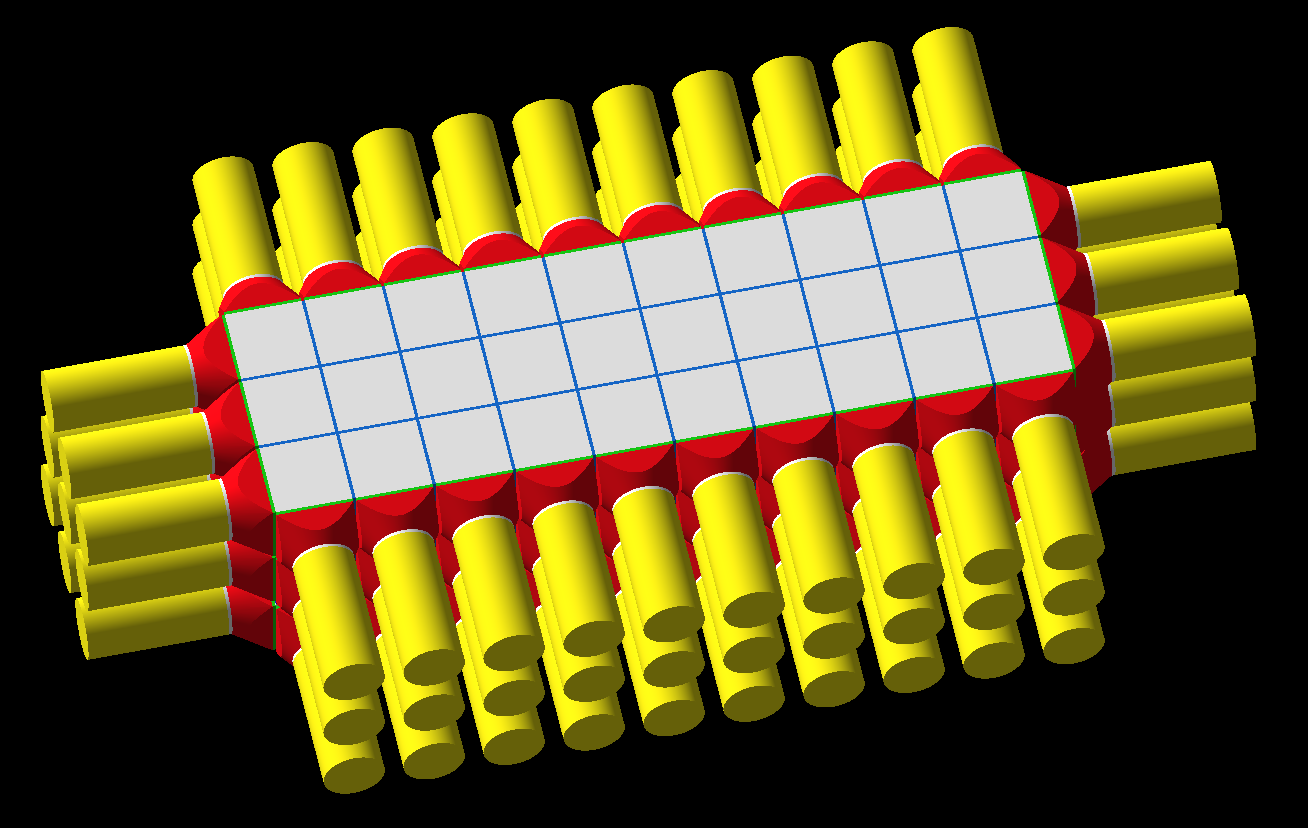
\includegraphics[width=\textwidth]{currentfig/numbera4.eps} % 单图
\end{figure}
\end{column}
\end{columns}
\begin{columns}
\begin{column}{.3\textwidth}
\begin{figure}
\centering
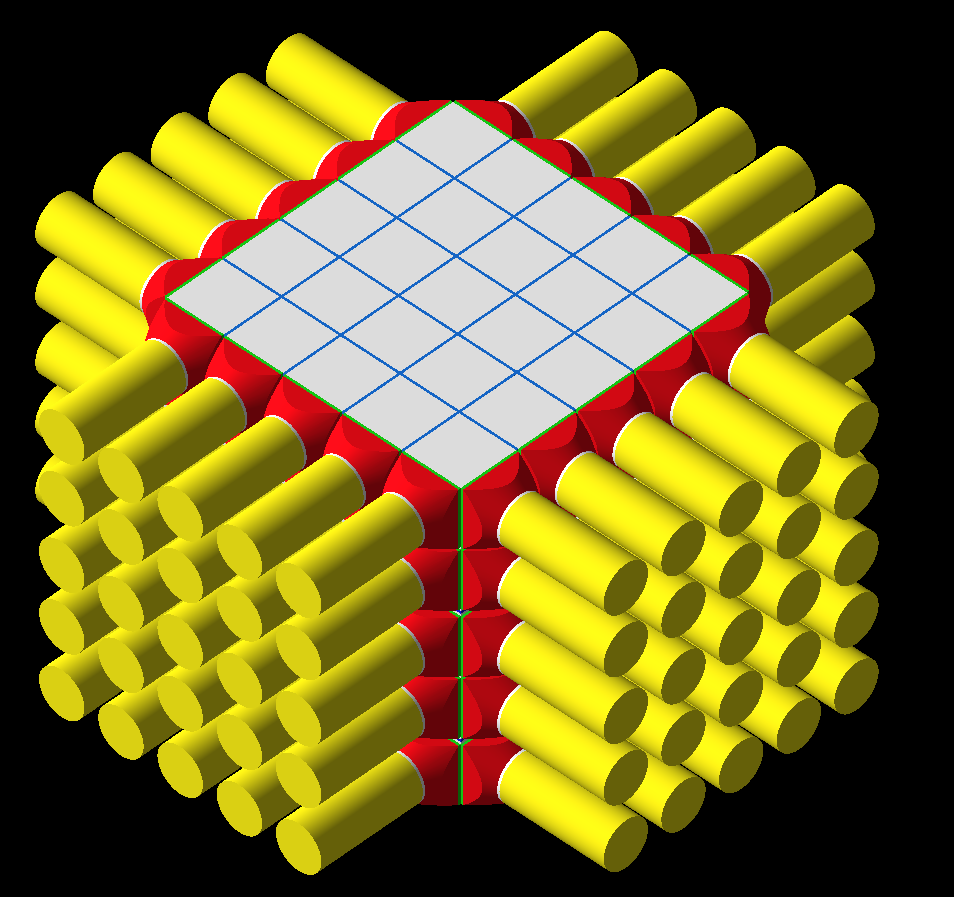
\includegraphics[width=\textwidth]{currentfig/numbera1.eps} % 单图
%\label{fig:wave2d}
%\caption{geometry of detector}
\end{figure}
\end{column}
\begin{column}{.3\textwidth}
\begin{figure}[!tbp]
\centering
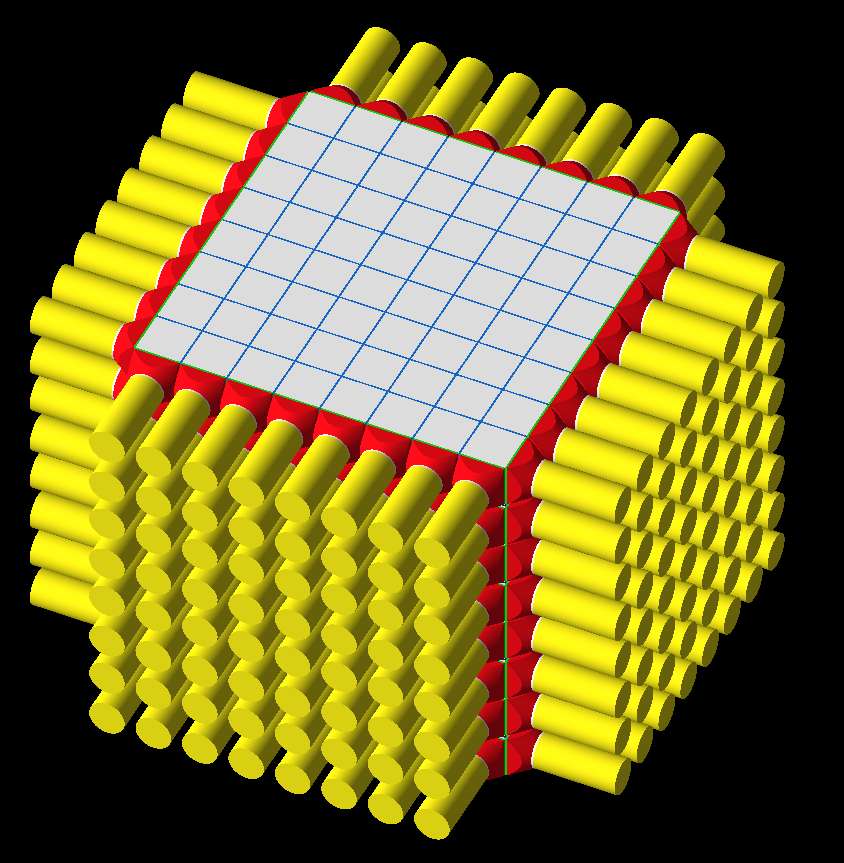
\includegraphics[width=.9\textwidth]{currentfig/numbera2.eps} % 单图
%\caption{geometry of detector}
\end{figure}
\end{column}
\begin{column}{.36\textwidth}
\begin{figure}[!tbp]
\centering
\includegraphics[width=.9\textwidth]{currentfig/numbera3.eps} % 单图
%\caption{geometry of detector}
\end{figure}
\end{column}
\end{columns}
\end{frame}
%%%%%%%%%%%%%%%%%%%%%%%%%%%%%%%%%%%%%%%%%%%%%%%%%%%%%%%%%%%%

\begin{frame}{THERMAL NEUTRON DETECTOR}
\begin{itemize}
\item the neutron detector EJ-426.
\item flat white thin sheet,$^6{Li}F:$(ZnS:Ag)
\end{itemize}
detection princeple:
\begin{equation}
^6Li+^1n\rightarrow^3H+^4He+4.78MeV
\end{equation}
The resulting triton and alpha particle are detected by ZnS:Ag phosphor with the broad blue fluorescent spectrum.
\begin{columns}
\begin{column}{.5\textwidth}
\begin{figure}
\centering
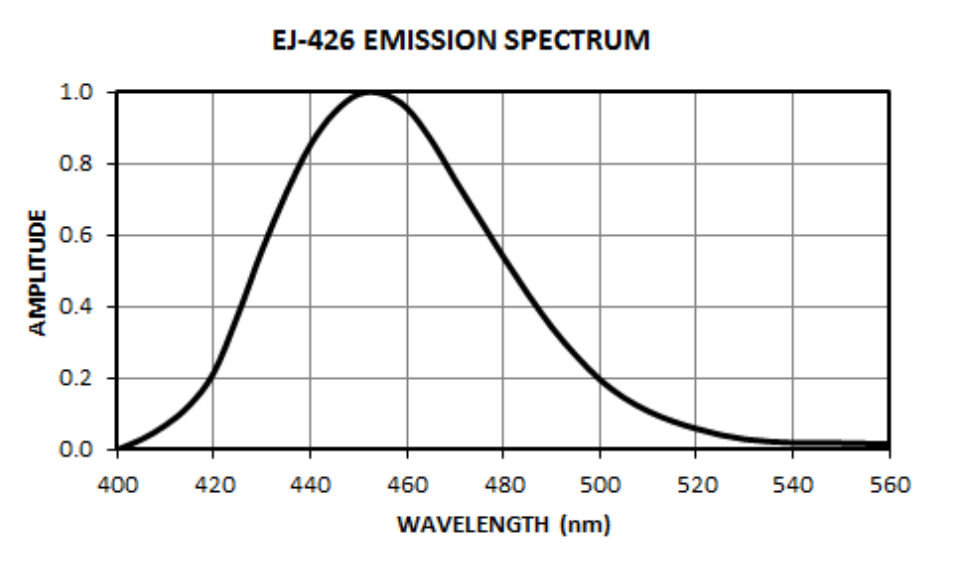
\includegraphics[width=\textwidth]{currentfig/ej426spec.png} % 单图
%\label{fig:wave2d}
%\caption{geometry of detector}
\end{figure}
\end{column}
\begin{column}{.5\textwidth}
\begin{figure}[!tbp]
\centering
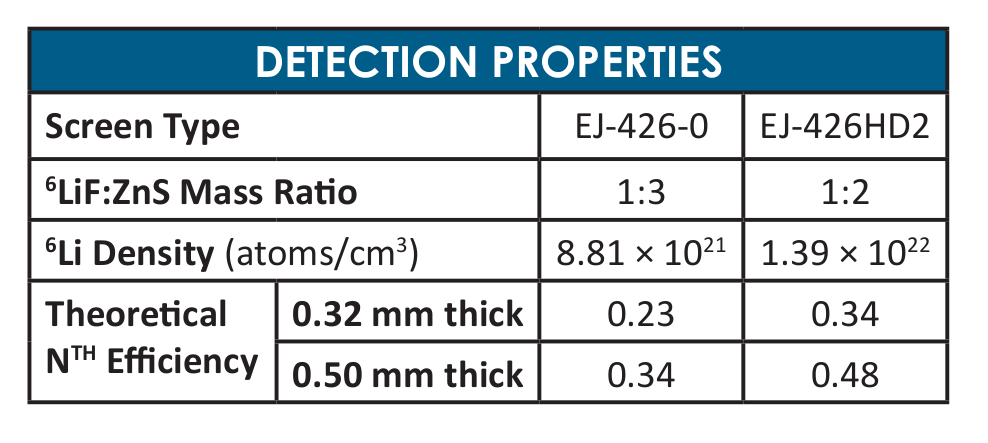
\includegraphics[width=.99\textwidth]{currentfig/ej426formula.png} % 单图
%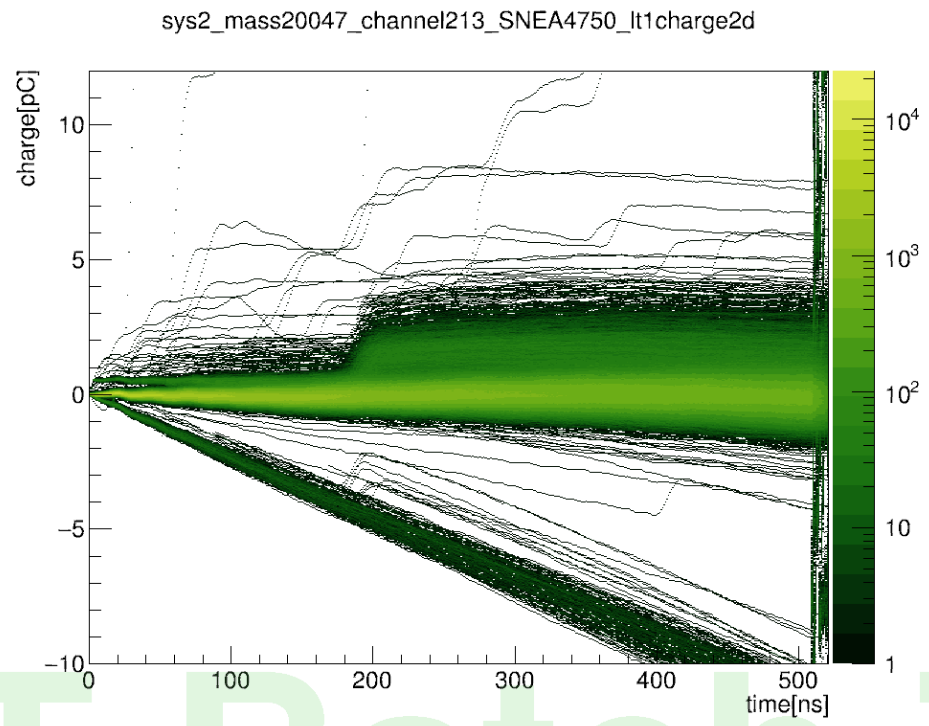
\includegraphics[width=\textwidth]{figures/baseline2d.png} % 单图
%\caption{geometry of detector}
\end{figure}
\end{column}
\end{columns}
\end{frame}
%%%%%%%%%%%%%%%%%%%%%%%%%%%%%%%%%%%%%%%%%%%
\begin{frame}{parameter adjustment}
\begin{enumerate}
\item choose the formula: EJ-426-0 or EJ-426HD2 ?
\item switch the thickness: 0.32mm or 0.5mm?
\item sheet size: 60mm$\times$ 60mm?
\item do we need backing material?
\end{enumerate}
\begin{figure}
\centering
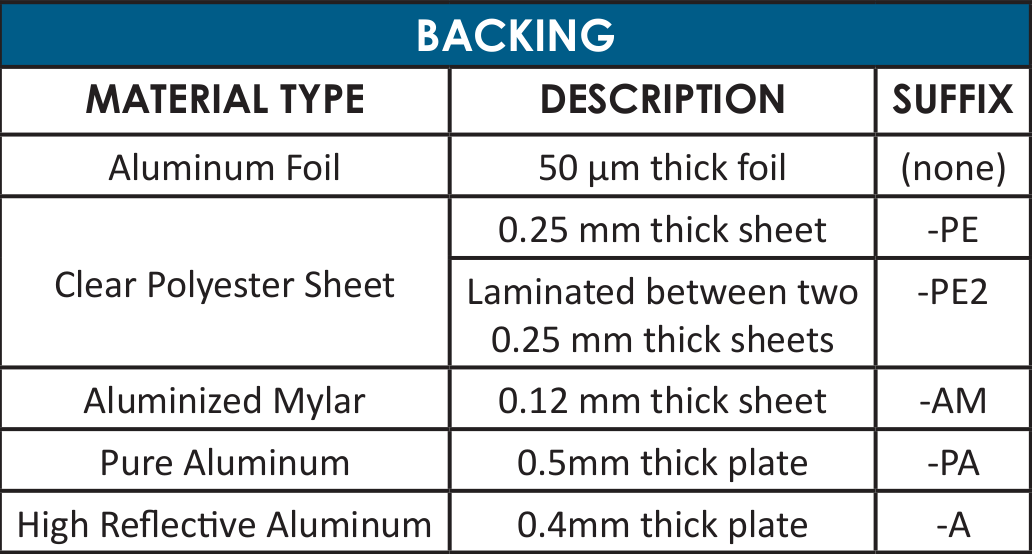
\includegraphics[width=0.64\textwidth]{currentfig/backing.png} % 单图
%\caption{108}
\end{figure}
\end{frame}

%%%%%%%%%%%%%%%%%%%%%%%%%%%%%%%%%%%%%%%%%%%
\begin{frame}{next to be done}
\begin{itemize}
\item detector construction \alert{.}
\begin{itemize}
\item add remain geometry [lightguides and PMTs].
\item attach correct material to each logical volume.
\item other components
\end{itemize}
\item adjustment of physis list
\begin{itemize}
\item  about scitillator material and their \alert{optical properties}
\item  optical performance of lightguides
\item  response of PMT [SiPM]
\item optical boundaries
\end{itemize}

\item add different primary \alert{paticle sources}\\
\begin{itemize}
\item alter the particle type,position,momentum,energy etc.\\
\item  use gps to control theparticle source
\end{itemize}
\item sensitive detector and scoring
\item more useractions for output and analyze.
\end{itemize}
\end{frame}
%%%%%%%%%%%%%%%%%%%%%%%%%%%%%%%%%%%%%%%%%%%
\begin{frame}{ update of work}
	\textbf{finished}
	\begin{itemize}
		\item finish the geometry.
\item finish the material
		\item add GPS
\item add sensitive detector (SD)
\item priliminary analyze codes
	\end{itemize}
	\hrule{\textwidth}
	\vspace{.8cm}
	\textbf{next to be done}
	\begin{itemize}
		\item more details about the optical photons(optical properties and optical boundaries)
		\item update the analyzing class
	\end{itemize}
\end{frame}
%%%%%%%%%%%%%%%%%%%%%%%%%%%%%%%%%%%%%%%%%%%
\begin{frame}{ material of detector components}
\begin{itemize}
	\item gamma scintillator:EJ-200   \\
		Base: Polyvinyl toluene \quad  formula : [CH2CH(C6H4CH3)]n
\begin{columns}
\begin{column}{.23\textwidth}
\begin{figure}
%\centering
	
\includegraphics[width=0.97\textwidth]{currentfig/Chemical_formula_for_polyvinyl_tolulene.png}
%\caption{108}
\end{figure}
\end{column}
\begin{column}{.73\textwidth}
	Density: 1.023 $g/cm^3$\\
	Refraction Index: 1.58 \\
	Light Output: No change from -60$\celsius $ to 20 $\celsius$
\end{column}
\end{columns}
	\vspace{.5cm}
	\hrule{\textwidth}
	\vspace{.5cm}

	\item thermal neutron scintillator:EJ-426HD2\\
	$^6LiF:ZnS \ Mass Ratio 1:3$\\
		$^6Li $ Density(atoms/cm$^3$)  : 1.39$\times 10^{22}$\\
		$^6$Li enriched to minimum of 95 atom percent.
\end{itemize}
%	light guide:  H-K9L\\
%	density: 2.52 g/cm3\\
\end{frame}
%%%%%%%%%%%%%%%%%%%%%%%%%%%%%%%%%%%%%%%%%%%
\begin{frame}{ details about detector components}
	\begin{enumerate}
		\item material of lightguide:  H-K9L
		\item  material of gaps between scintillators: air
		\item  PMTs around the scintillators as sensitive detectors
		\item currently PMTs work as ideal detectors with 100\% PDE
	\end{enumerate}
\end{frame}
\begin{frame}{density of EJ-426}
	formula:	($^6LiF$)(ZnS:Ag) \qquad density of $^6$Li : 1.39*10$^{22}$ atoms/cm$^3$\\
atomic mass of $^6$Li: 6.0151amu\\
atomic mass of $^7$Li: 7.0160amu \\
atomic mass of Fluorine	: 18.9984amu \\
$^6$LiF:ZnS Mass Ratio: 1:2 \\
%atomic mass of Zinc: 65.39amu \\
%atomic mass of Sulfur: 32.065amu \\
%atomic mass of Silver: 107.8682amu \\
 density:(6.0151*.95+7.0160*0.05+18.9984)*3*0.139/6.022=1.7355/cm$^3$

\end{frame}

%%%%%%%%%%%%%%%%%%%%%%%%%%%%%%%%%%%%%%%%%%%
%\vspace{-.5cm}
%%%%%%%%%%%%%%%%%%%%%%%%%%%%%%%%%%%%%%%%%%%
%\begin{frame}{Testing results output}
%\begin{figure}
%\centering
%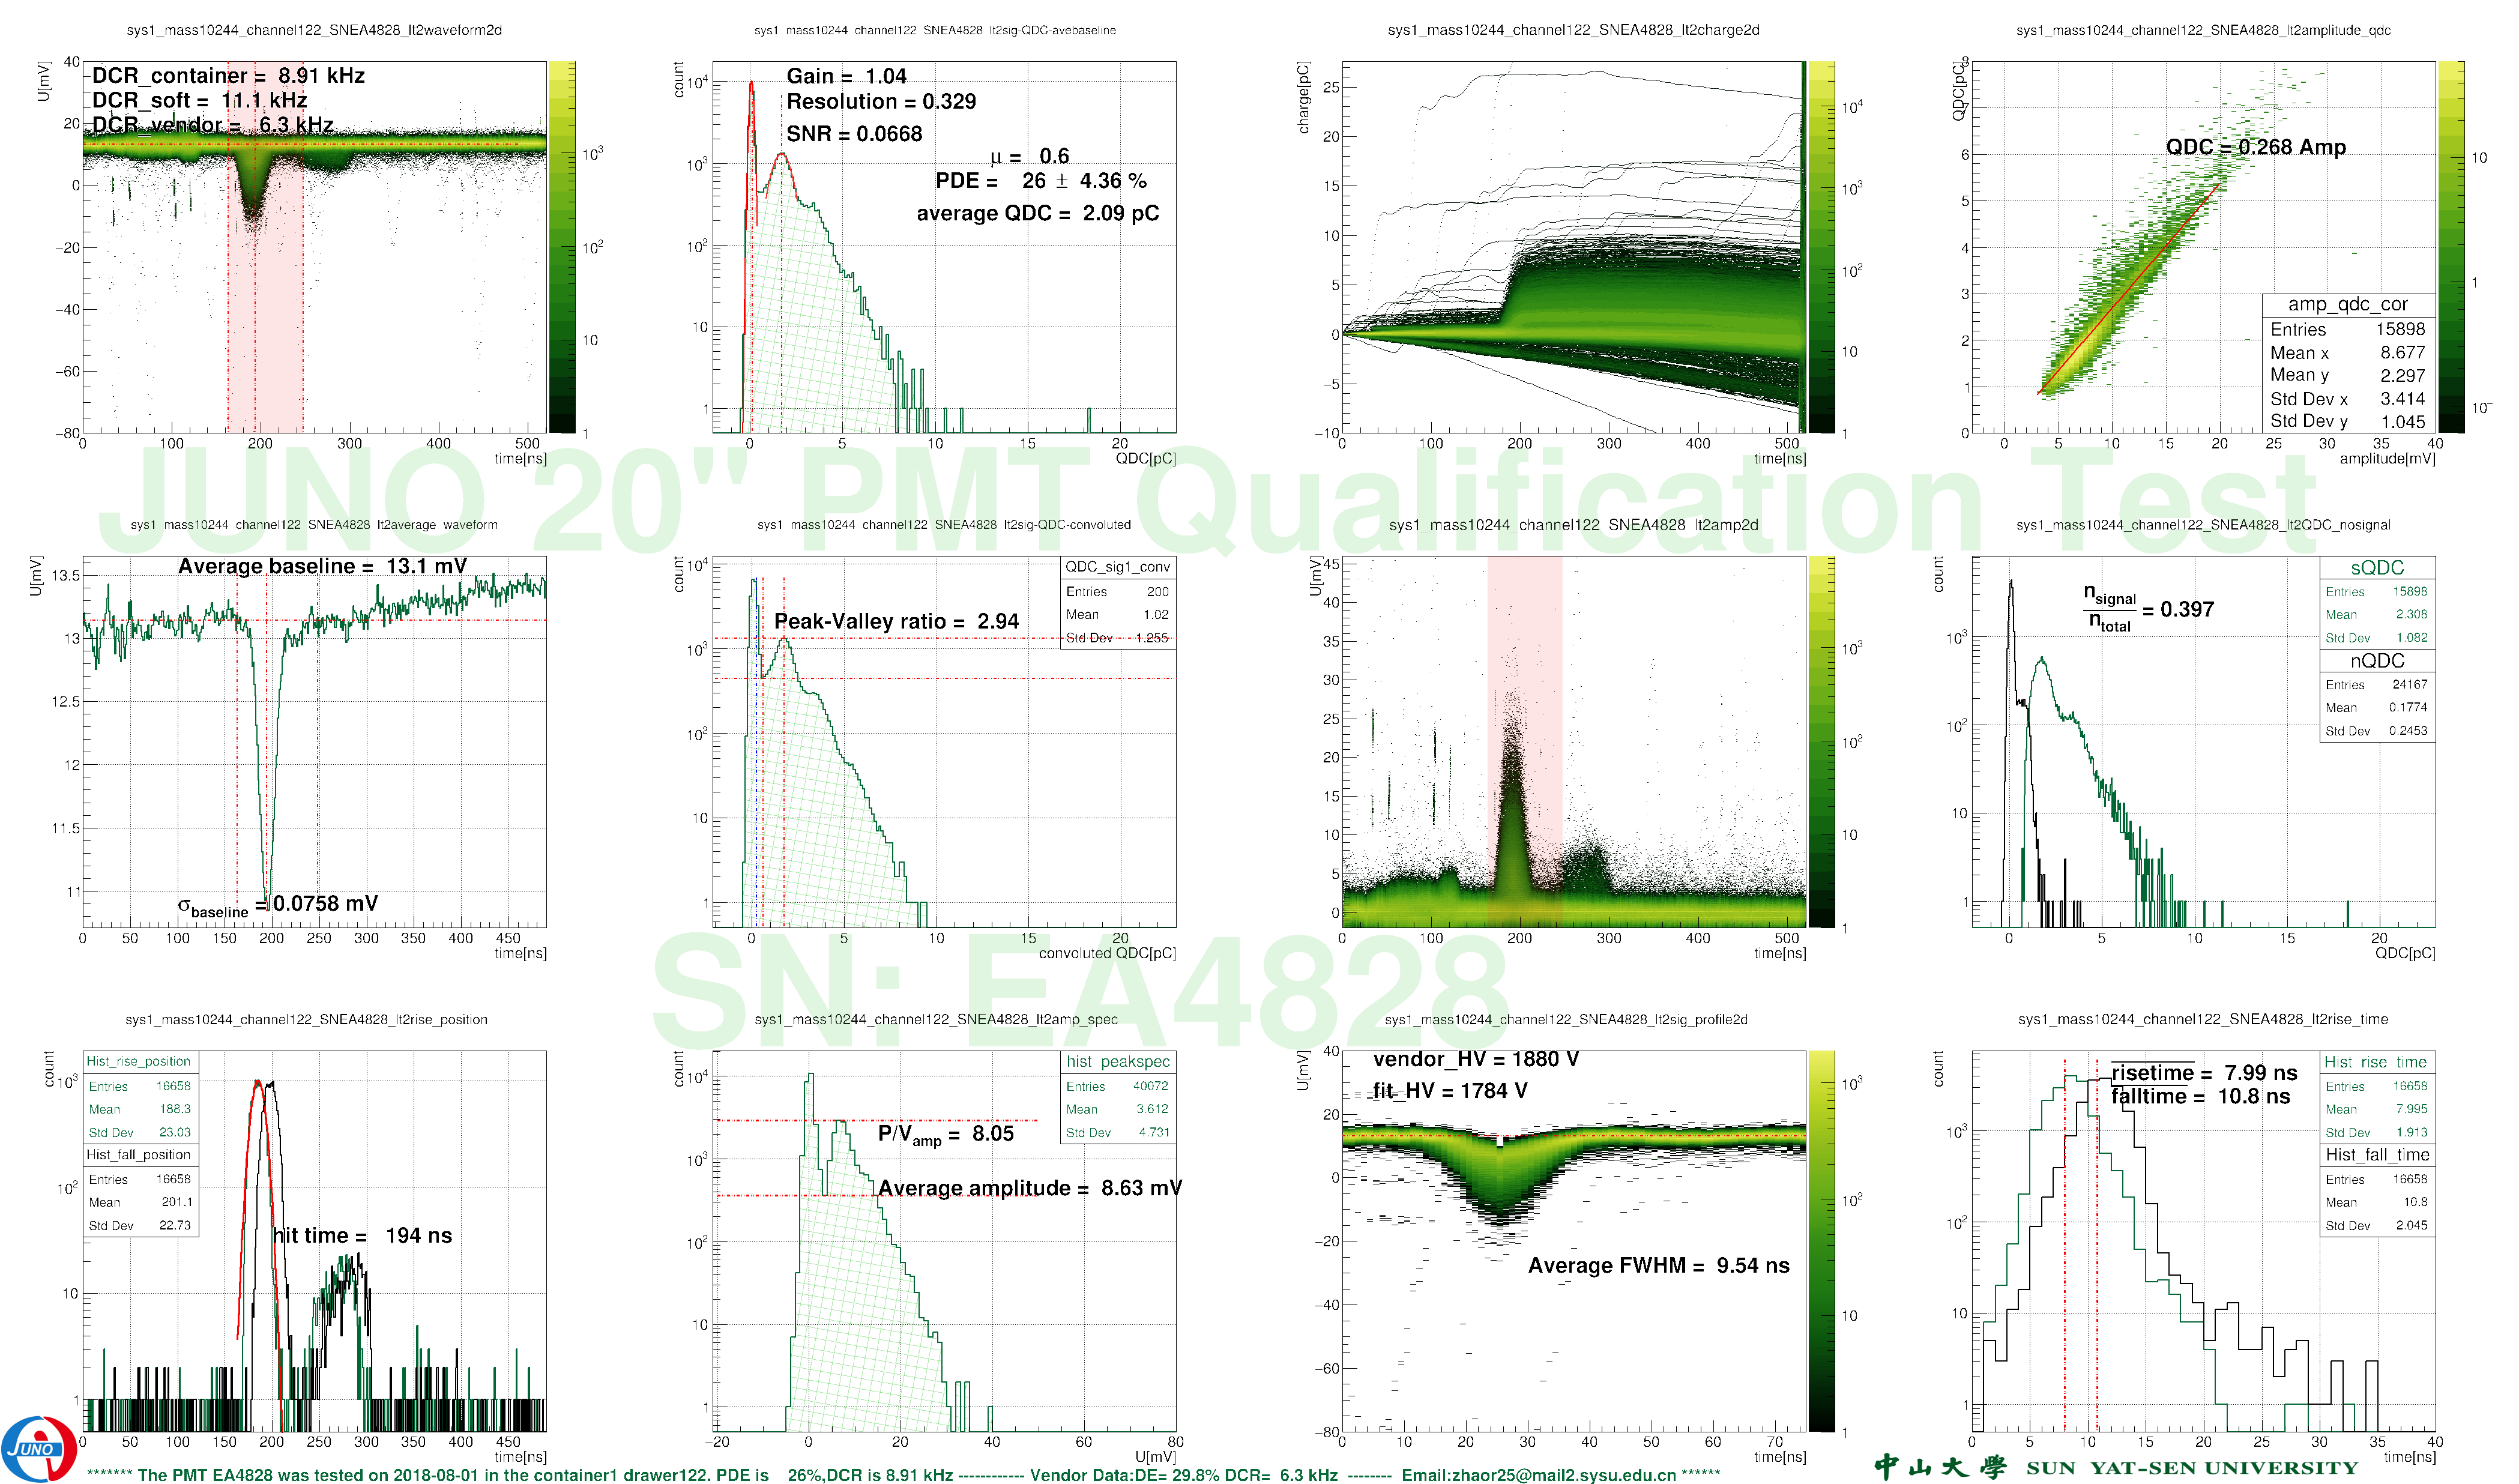
\includegraphics[width=1.0\textwidth]{figures/sys1_mass10244_channel122_snEA4828_lt2.png}
%\end{figure}
%\end{frame}
%%%%%%%%%%%%%%%%%%%%%%%%%%%%%%%%%%%%%%%%%%%%
%\begin{frame}{PMT testing report-pass}
%We have generated testing report for each qualified PMT.
%\vspace{-.2cm}
%\begin{figure}
%\centering
%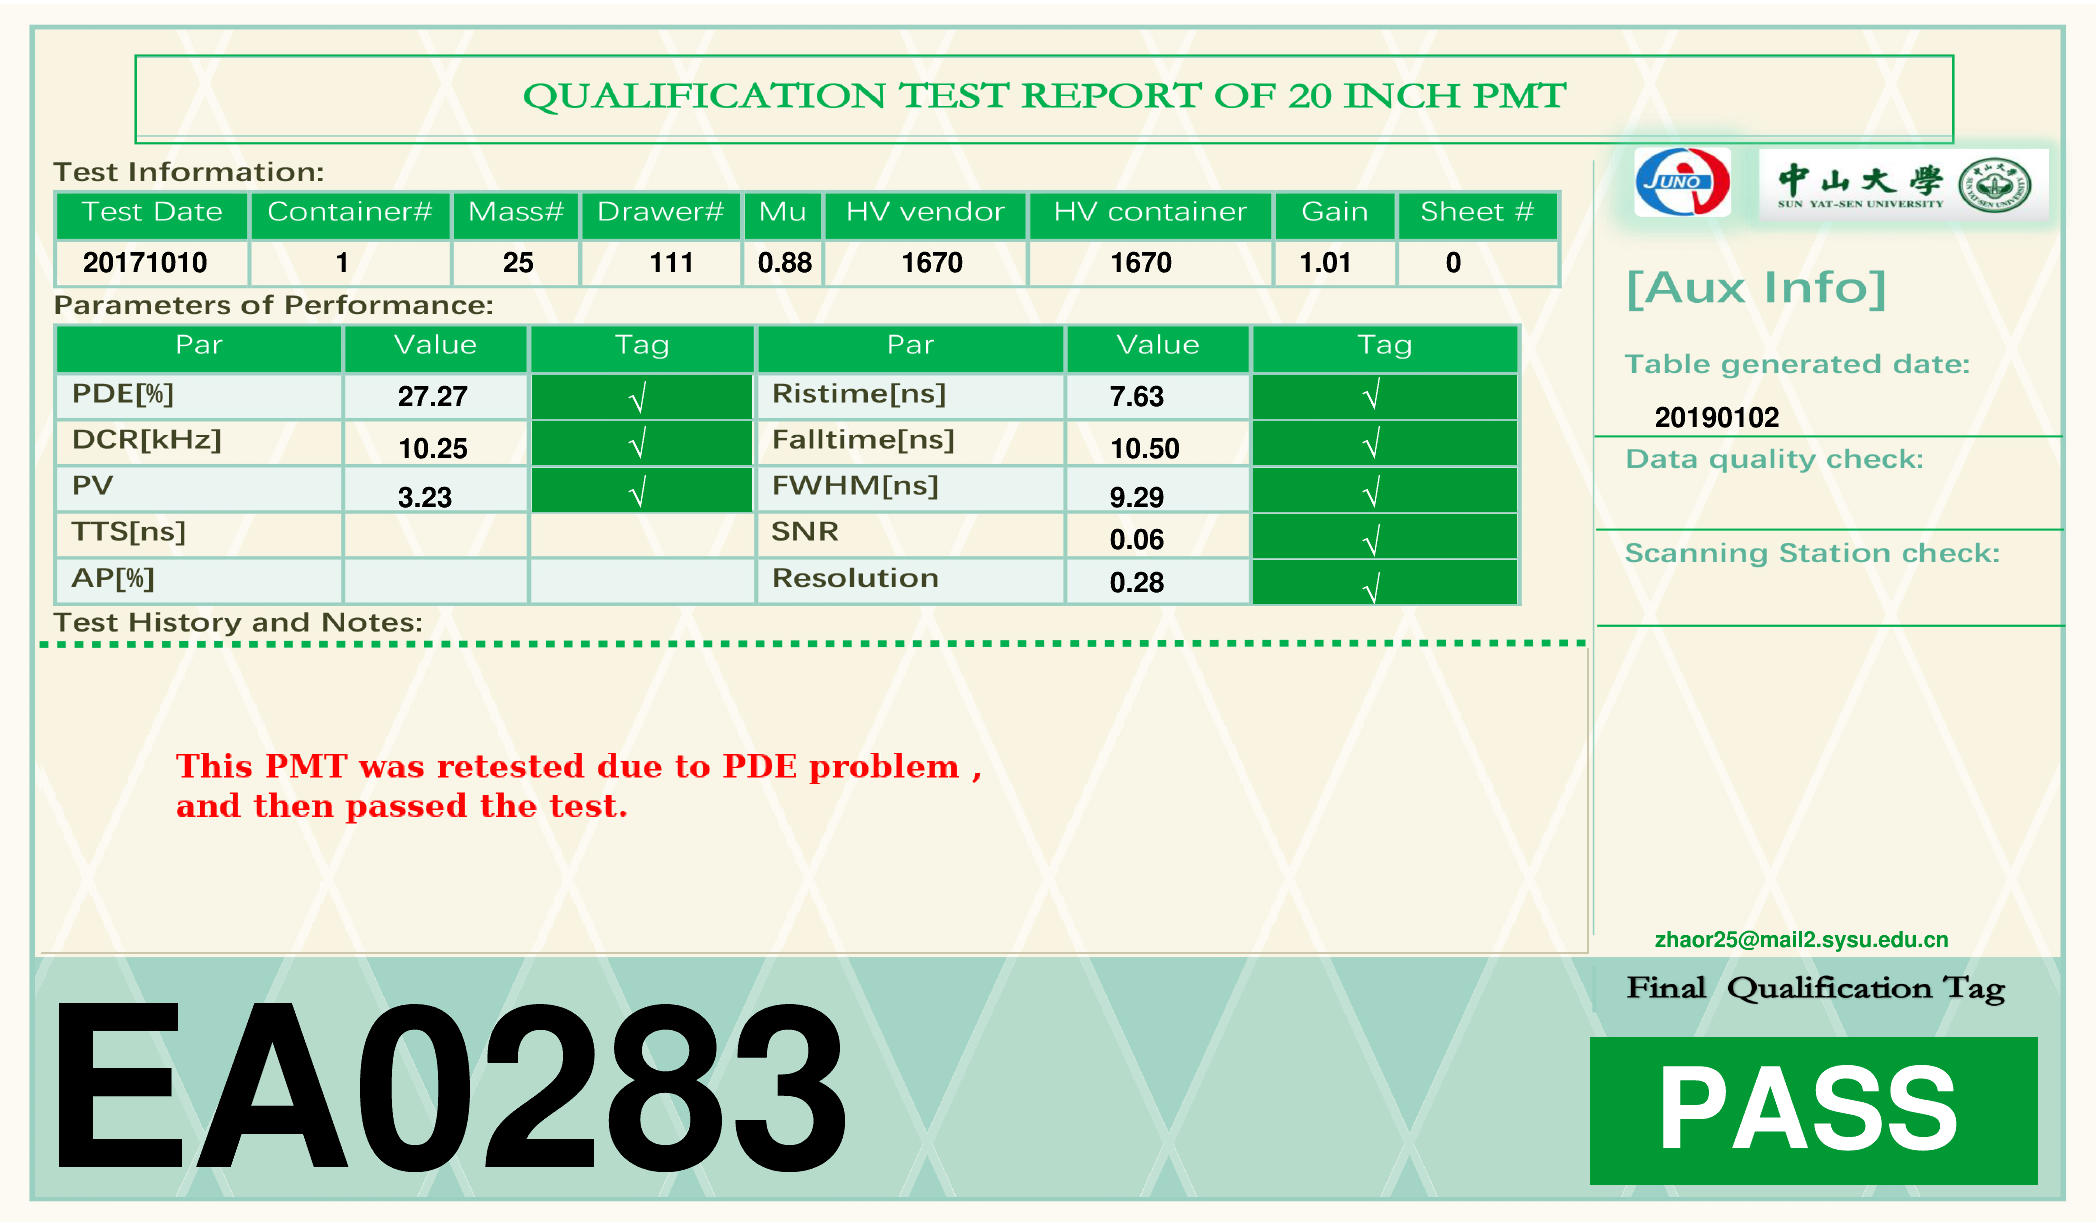
\includegraphics[width=1.0\textwidth]{figures/SN_EA0283_pde1_dcr1_HV1_pv1_rt1_tag1.png}
%\end{figure}
%\end{frame}
%%%%%%%%%%%%%%%%%%%%%%%%%%%%%%%%%%%%%%%%%%%
%\begin{frame}{calibration of each drawer}
%Generally, we put several PMTs with known PDE value\footnote{or QE value}  into one drawer and linearly fit the PDE-$\mu_{test}$ data to get \alert{drawer$_{factor}$}.
%\vspace{.5cm}
%\hrule{\textwidth}
%\vspace{.5cm}
%
%While an alternative way to access the drawer$_{factor}$ is fitting PDE-$\mu_{test}$ data {\color{red}from all the PMTs tested in one drawer rather than the mannual selected ones.} Then once we finish one PMT test in a drawer we will get one more statistical sample in the PDE-$\mu_{test}$ fitting, and we could expect that the fitted drawer$_{factor}$ will get more stable as we testing more PMTs.
%
%\vspace{.5cm}
%The advantage of this "self-calibration" method is that we could {\color{red}decrease the statistical error as much as possible}; and the remained fluctuation of drawer$_{factor}$ can be the system error.
%\end{frame}
\section{physcis and scoring}
%\begin{frame}{一个抽屉的刻度结果}
%随着测试PMT数量的增加,拟合统计误差逐渐减小,$drawer_{factor}$的拟合结果趋于稳定(更多抽屉拟合结果见back-up部分)。
%\begin{figure}
%\centering
%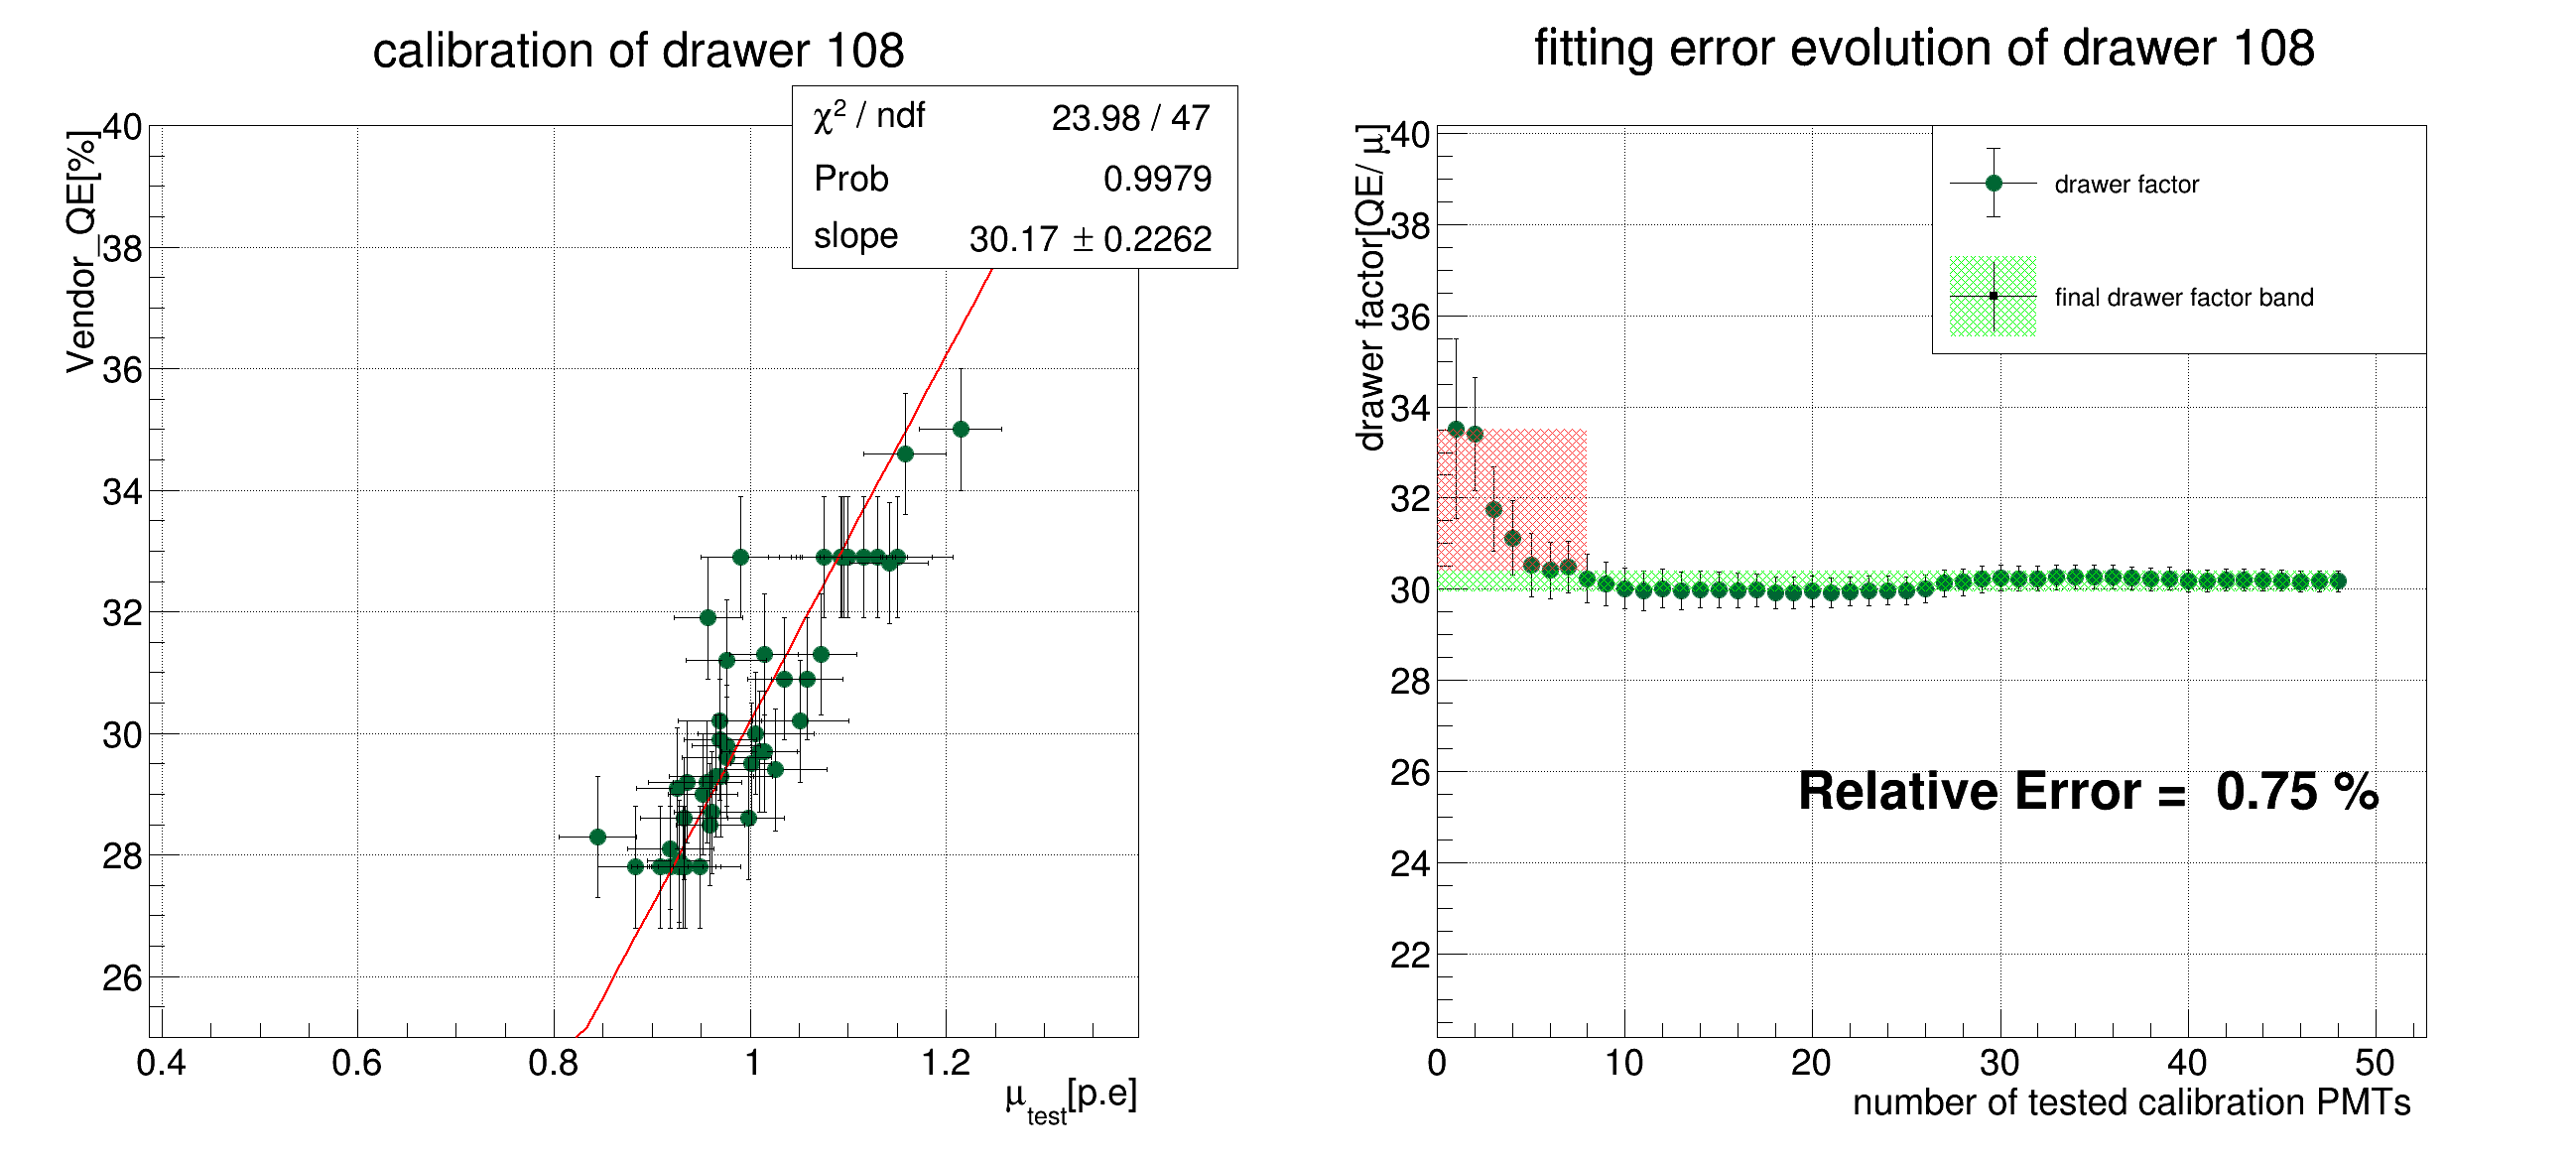
\includegraphics[width=0.98\textwidth]{sta101-7} % 单图
%\caption{108抽屉的$drawer_{factor}$拟合结果}
%\end{figure}
%\end{frame}
%%%%%%%%%%%%%%%%%%%%%%%%%%%%%%%%%%%%%%%%%%%
%\begin{frame}{physics}
%%Typical signal waveform when working @$gain=10^7$
%\begin{itemize}
%\item light yield of scitillator
%\item response (PDE,time resolution) of SiPM or PMT
%\item consideration of calibration using gamma and neutron source
%\end{itemize}
%\begin{columns}
%\begin{column}{.485\textwidth}
%\begin{figure}
%\centering
%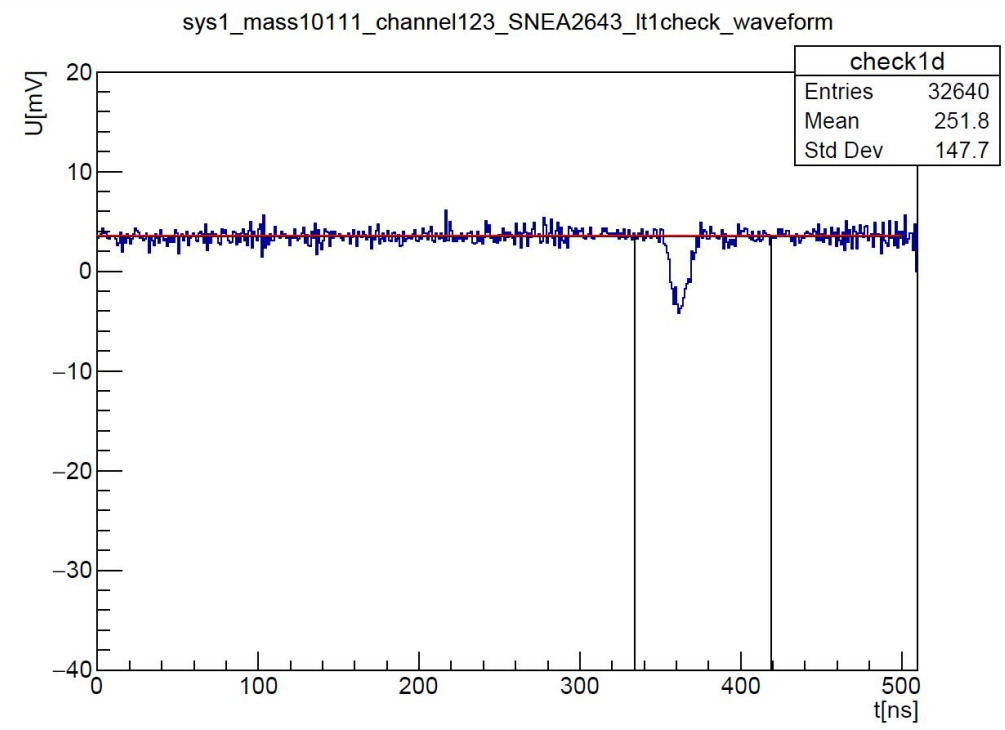
\includegraphics[width=\textwidth]{figures/hamwave.png} % 单图
%%\label{fig:wave2d}
%\caption{single photon signal waveform of HAMAMATSU PMT}
%\end{figure}
%\end{column}
%\begin{column}{.5\textwidth}
%\begin{figure}
%\centering
%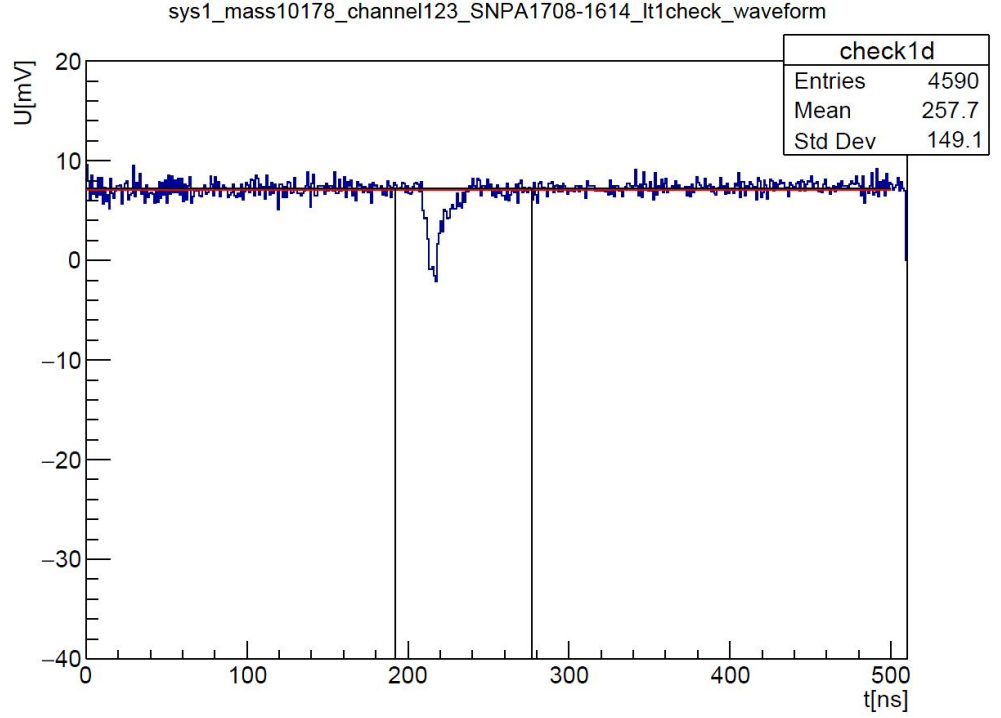
\includegraphics[width=\textwidth]{figures/mcpwave.png} % 单图
%%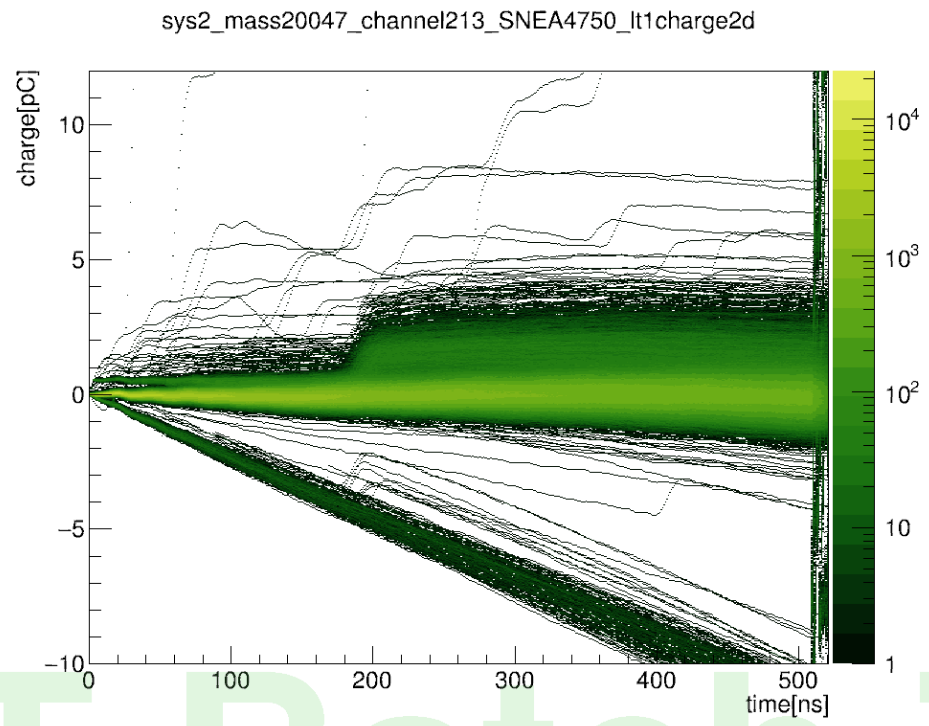
\includegraphics[width=\textwidth]{figures/baseline2d.png} % 单图
%\caption{single photon signal waveform of NNVT PMT}
%\end{figure}
%\end{column}
%\end{columns}
%\end{frame}
%%%%%%%%%%%%%%%%%%%%%%%%%%%%%%%%%%%%%%%%%%%
%~~!!!!!!!!!!!!!!!!!!put two figures to illustrate!!!!!
\begin{frame}{sensitive detector}
%choose the surface of SiPM as sensitive detector, record the number of photons, hit time
%\begin{columns}
%\begin{column}{.47\textwidth}
%\begin{figure}
%\centering
%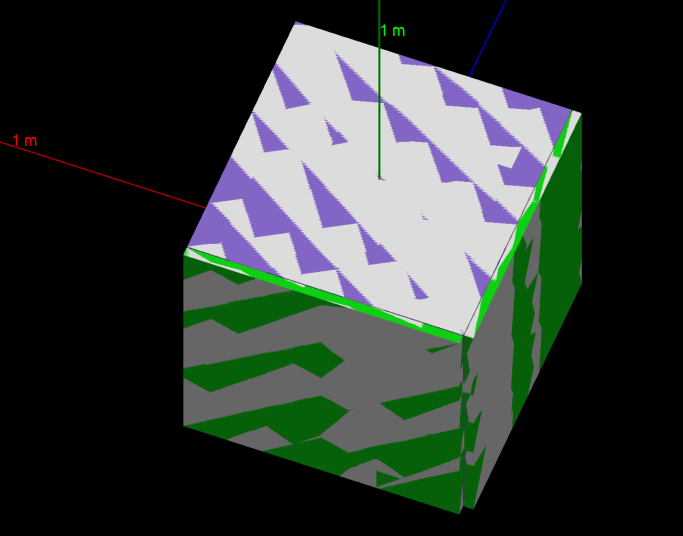
\includegraphics[width=\textwidth]{currentfig/geom1.png} % 单图
%%\label{fig:wave2d}
%\caption{i}
%\end{figure}
%\end{column}
%\begin{column}{.5\textwidth}
%\begin{figure}
%\centering
%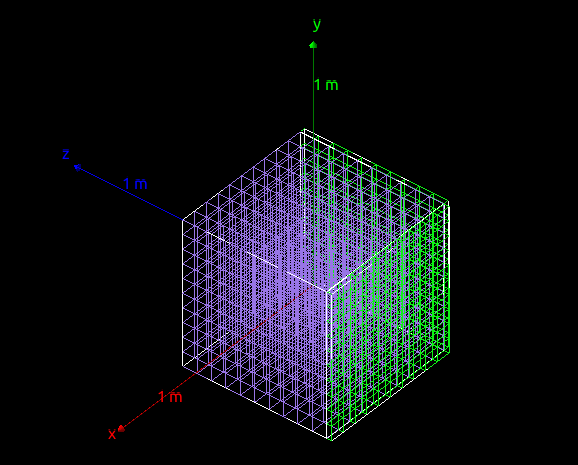
\includegraphics[width=\textwidth]{currentfig/geom2.png} % 单图
%%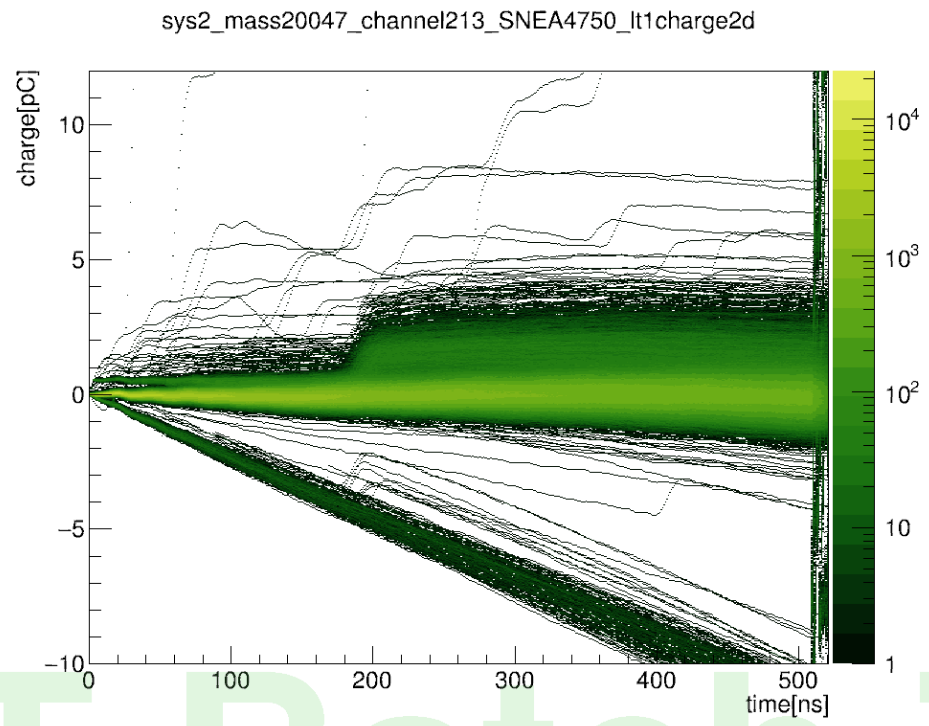
\includegraphics[width=\textwidth]{figures/baseline2d.png} % 单图
%\caption{simulation results}
%\end{figure}
%\end{column}
%\end{columns}\item
\begin{enumerate}
	\item optical photon with single wavelength(energy)
	\item PMT record the time and count of photon hits.
	\item  do I need to attach SD to scintillators inside?
\end{enumerate}
\end{frame}

%%%%%%%%%%%%%%%%%%%%%%%%%%%%%%%%%%%%%%%%%%%
\begin{frame}{optical simulation part}
	response curve v.s photon energy(wavelength)
	\begin{itemize}
		\item scintillator emission spectrum
		\item reflectivity of materials
		\item refractive index
		\item attenuation length
		\item PMT detection effictioncy
	\end{itemize}
	active the rise time. the scintillation process.
	 absorption and re-emission of photons; Boundary Process
\end{frame}
%%%%%%%%%%%%%%%%%%%%%%%%%%%%%%%%%%%%%%%%%%%
\section{simulation output }
\begin{frame}{play around- the 2D case}
	

\end{frame}
%%%%%%%%%%%%%%%%%%%%%%%%%%%%%%%%%%%%%%%%%%%
%\begin{frame}{number of photons}
%\begin{frame}{todo list}
%\begin{itemize}
%\item  finish the sensitive detector and scoring part of simulation
%\item add specified physics list
%\item add more useraction
%\item simulation 1 dimention performance
%\end{itemize}
%\begin{equation}
%PDE_{c}=\mu_{test}\times drawer_{factor}
%\end{equation}
%\begin{equation}
%PDE=PDE_{c}.f_{cs}+constant
%\label{pde_formula}
%\end{equation}
%%根据公式\ref{pde_formula},通过$\mu_{test}$以及抽屉因子即可算出集装箱自己的PDE结果$PDE_c$。假设集装箱系统和扫描站对同一只PMT的测量结果是正比关系\footnote{参考王俊和王耀光的模拟结果},通过拟合线性参数$f_{cs}$可以算出最终的PDE。
%\vspace{.5cm}
%\hrule{\textwidth}
%\vspace{.5cm}

%\end{frame}
%%%%%%%%%%%%%%%%%%%%%%%%%%%%%%%%%%%%%%%%%%%
%%%%%%%%%%%%%%%%%%%%%%%%%%%%%%%%%%%%%%%%%%%%%%%%%%%%%%%%%%%%%%%%%%%%
%\begin{frame}{PDE计算结果}
%将MCP-PMT的高量子效率分开处理,统计集装箱1测量到的MCP-PMT的PDE结果\footnote{更新到2018-10-17的测试结果}:
%%\hrule{\textwidth}
%\begin{columns}
%\begin{column}{.56\textwidth}
%\begin{figure}
%\centering
%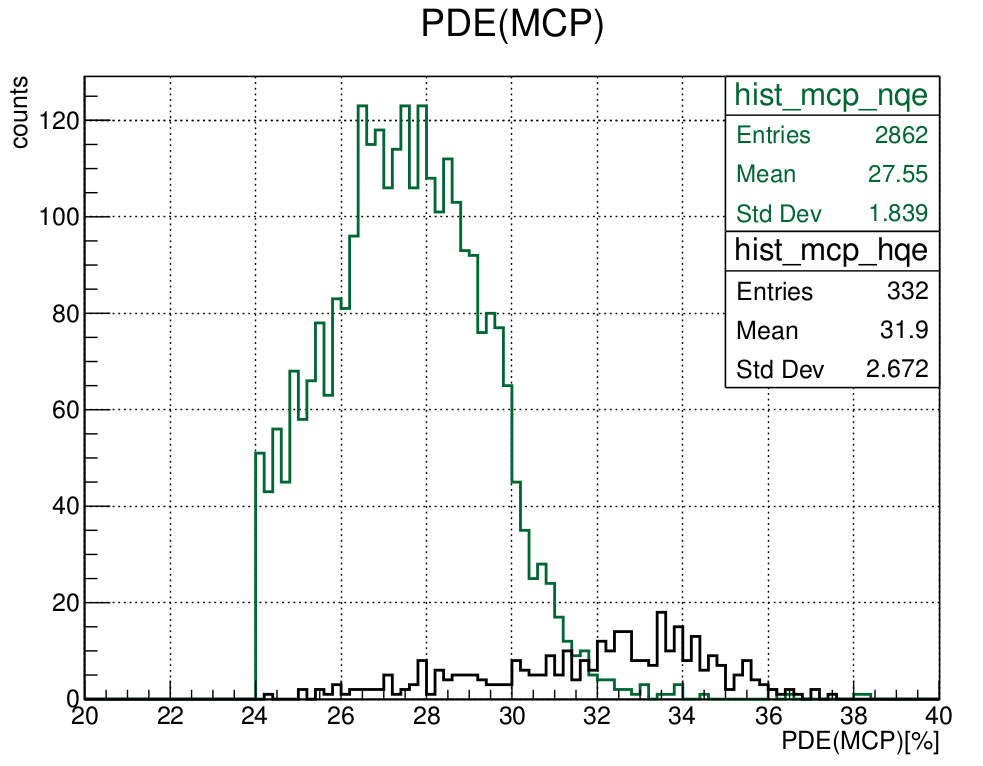
\includegraphics[width=\textwidth]{mcppde}
%\end{figure}
%\end{column}
%\begin{column}{.4\textwidth}
%\alert{MCP的高量子效率版本PDE相对增加了15.8\%}
%\vspace{.5cm}
%\hrule{\textwidth}
%\vspace{.5cm}
%PDE 的统计结果和现场算法得到的结果一致。\\
%MCP:27.5\leftrightarrow \alert{27.55}\\
%HAMAMATSU:28.5\leftrightarrow \alert{28.56}
%\end{column}
%%\end{figure}
%\end{columns}
%\end{frame}
%%%%%%%%%%%%%%%%%%%%%%%%%%%%%%%%%%%%%%%%%%%%%%%%%%%%%%%%%%%%%%%
%%%%%%%%%%%%%%%%%%%%%%%%%%%%%%%%%%%%%%%%%%%%%%%%%%%%%%%%%%%%%%%
\section{summary}

\begin{frame}{summary}
\begin{itemize}
\item  almost finish simple detector geometry.
\item  other parts of simulation program still in progress.
\end{itemize}
\end{frame}

%\begin{frame}
%\centering {\zihao{0} \color{red} \calligra{谢谢}}
%\end{frame}

\begin{frame}
\centering {\zihao{0} \color{red} \calligra{BACK-UP}}
\end{frame}

%\begin{frame}[allowframebreaks]
%\frametitle{References}
%\scriptsize
%\bibliographystyle{authordate1}
%\bibliography{R-GLMM-pkgs}
%\end{frame}

\appendix

\section*{附录}
%%%%%%%%%%%%%%%%%%%%%%%%%%%%%%%%%%%%%%%%%%%%
%\begin{frame}{平均PDE}
%每个抽屉的平均PDE分布:
%\begin{figure}
%\centering
%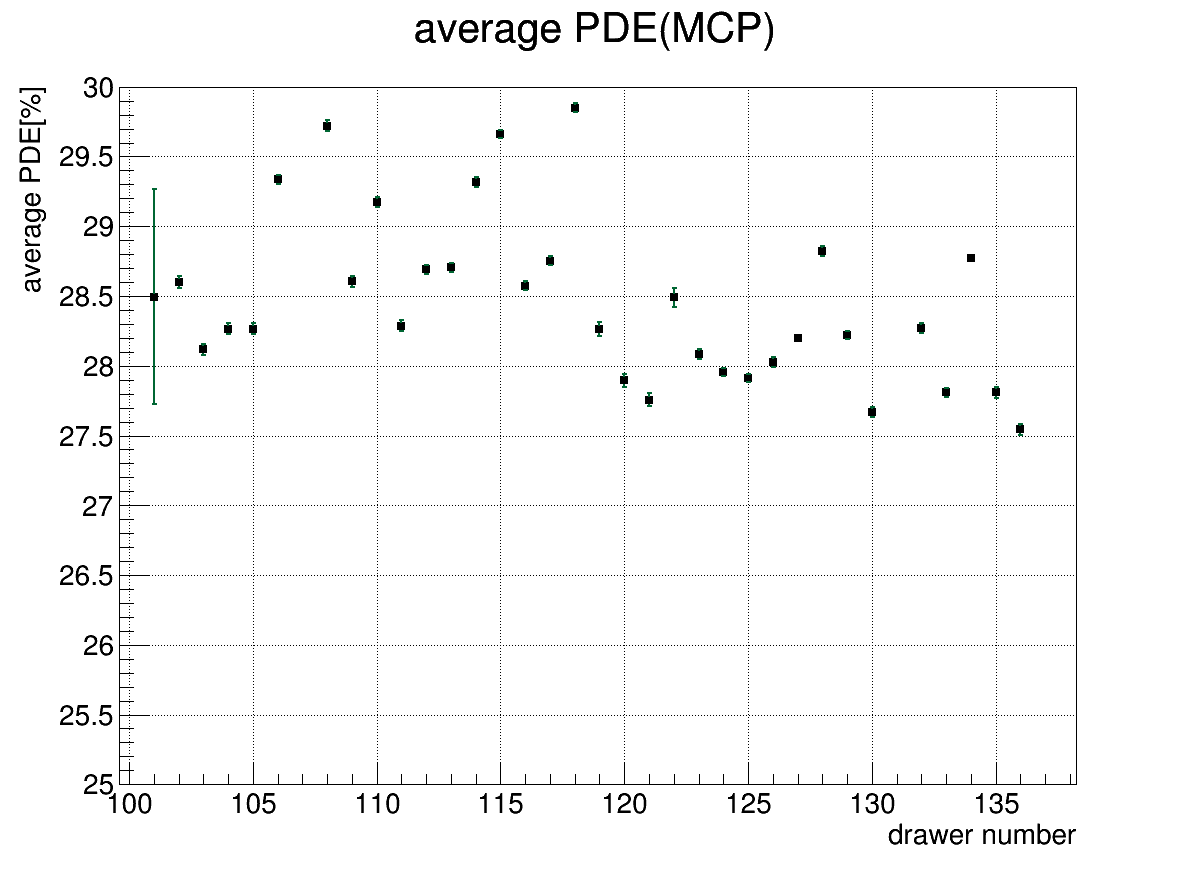
\includegraphics[width=0.88\textwidth]{dpde}
%\end{figure}
%\end{frame}
%% OpenBUGS  WinBUGS  JAGS
% library(R2OpenBUGS) # 2017-2-20 version 3.2-3.2
% library(R2WinBUGS) # 2015-07-29 version 2.1-21
% library(rjags) # 2016-02-19 version 4-6
% library(BRugs) # OpenBUGS 2017-06-26  version 0.9-0
% library(glmmBUGS) # Generalised Linear Mixed Models with BUGS and JAGS 2016-09-22 version 2.4.0
% library(R2jags) # Using R to Run 'JAGS'  2015-08-23	 version 0.5-7

% network
	% diagram DiagrammeR DiagrammeRsvg
 % library(help=graph)

 % library(help=Rgraphviz)
 % library(help=igraph)


%\begin{frame}{Ack}
%\begin{itemize}
%\item[\faGithub] \href{https://github.com/Cloud2016}{Cloud2016} \faAt Github
%\item[\aiOverleaf] \href{https://www.overleaf.com/}{Xiangyun} \faAt Overleaf
%\item[\aiarXiv] \href{https://arxiv.org/}{arXiv}
%\end{itemize}
%\end{frame}

\end{document}
